% !TeX root = ../main.tex
% !TeX encoding = utf8

% Librerías TikZ necesarias para los organigramas
\usetikzlibrary{positioning, arrows.meta, calc}

\chapter{Descripción de las partes de la organización}
% Responsable: Julián Carrión Tovar
% Secciones del índice: 2. Descripción de las partes de la organización

En este capítulo se analiza la sucursal de Motril como unidad organizativa autónoma.
Las instancias superiores ---Consejo de Administración, Comisión Ejecutiva y Director
de Área--- se tratan como entorno externo que impone objetivos y directrices, pero no
forman parte de la estructura interna de la sucursal. Se presentan dos organigramas:
uno que sitúa la sucursal en la jerarquía de CaixaBank (contexto externo) y otro de
su estructura interna, seguidos de la descripción de cada unidad o puesto.

% ===================================================================
\section{Organigrama de CaixaBank}
% ===================================================================

\subsection{Posición de la sucursal en la jerarquía del grupo}

A nivel corporativo, CaixaBank opera bajo la supervisión de un Consejo de Administración
formado por 15 consejeros [\ref{ref:cnmv}]. La gestión ejecutiva del grupo recae en el
Consejero Delegado, Gonzalo Gortázar Zapatero, quien ejerce sus funciones a través de
la Comisión Ejecutiva y de las distintas áreas corporativas especializadas ---Finanzas,
Riesgos, Tecnología, Recursos Humanos, Cumplimiento, entre otras---. La red comercial
se organiza territorialmente: cada \textbf{Director de Área} supervisa aproximadamente
18 sucursales de su zona geográfica, actuando como nivel intermedio entre la sede central
y las oficinas [\ref{ref:entrevista}].

La sucursal de Motril pertenece a esta red y rinde cuentas al Director de Área
correspondiente. La Figura~\ref{fig:organigrama-corp} ilustra este esquema. A efectos
del análisis estructural interno que sigue, todas las instancias representadas por
encima de la sucursal se consideran entidades externas.

\begin{figure}[htbp]
  \centering
  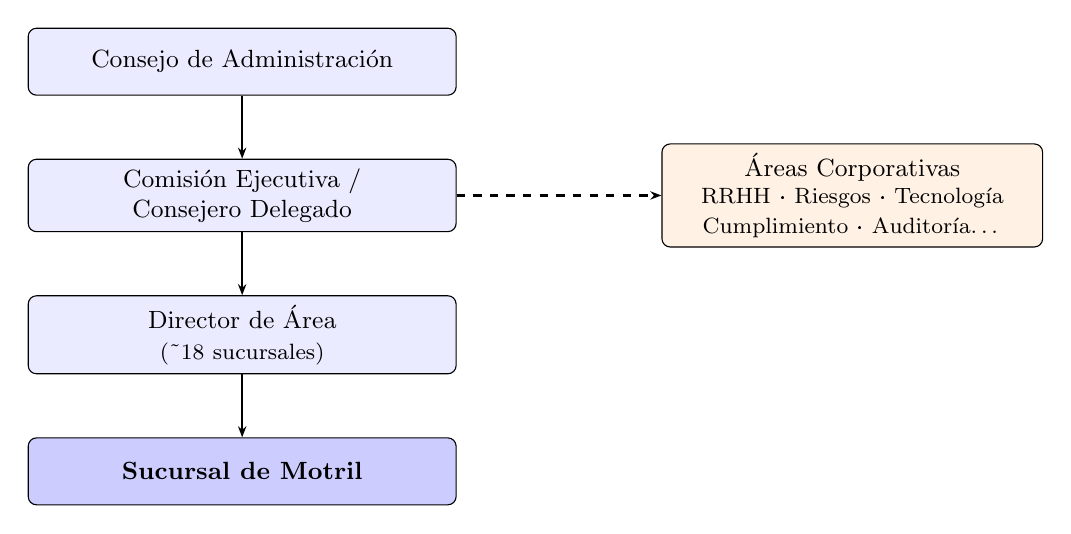
\begin{tikzpicture}[
    mainbox/.style = {
      rectangle, draw, rounded corners = 3pt,
      text width = 5.2cm, align = center,
      minimum height = 0.85cm, font = \small,
      fill = blue!8
    },
    staffbox/.style = {
      rectangle, draw, rounded corners = 3pt,
      text width = 4.6cm, align = center,
      minimum height = 0.85cm, font = \small,
      fill = orange!10
    },
    hibox/.style = {
      rectangle, draw, rounded corners = 3pt,
      text width = 5.2cm, align = center,
      minimum height = 0.85cm, font = \small\bfseries,
      fill = blue!20
    },
    arr/.style  = {-{Stealth[length=4pt]}, thick},
    darr/.style = {-{Stealth[length=4pt]}, thick, dashed}
  ]

  % Cadena jerárquica principal
  \node[mainbox] (ca)  {Consejo de Administración};
  \node[mainbox, below = 0.8cm of ca]  (ce)  {Comisión Ejecutiva /\\Consejero Delegado};
  \node[mainbox, below = 0.8cm of ce]  (da)  {Director de Área\\{\footnotesize (\textasciitilde18 sucursales)}};
  \node[hibox,   below = 0.8cm of da]  (suc) {Sucursal de Motril};

  % Bloque de áreas corporativas (derecha)
  \node[staffbox, right = 2.6cm of ce] (corp)
    {Áreas Corporativas\\{\footnotesize RRHH · Riesgos · Tecnología\\Cumplimiento · Auditoría…}};

  % Conexiones verticales
  \draw[arr]  (ca)  -- (ce);
  \draw[arr]  (ce)  -- (da);
  \draw[arr]  (da)  -- (suc);
  \draw[darr] (ce)  -- (corp);

  \end{tikzpicture}
  \caption{Posición de la sucursal de Motril en la jerarquía de CaixaBank (esquema simplificado).
    Fuente: elaboración propia a partir de [\ref{ref:cnmv}]
    y [\ref{ref:entrevista}].}
  \label{fig:organigrama-corp}
\end{figure}

\subsection{Organigrama interno de la sucursal de Motril}

La estructura interna de la sucursal presenta una particularidad relevante: los
\textbf{Gestores de Negocio} y los \textbf{Gestores Premier} dependen directamente de
la Directora, mientras que los \textbf{Gestores de Banca Particular} y los
\textbf{Gestores de Banca Personal} quedan bajo la supervisión de la Subdirectora.
La plantilla total asciende a \textbf{15 personas}, distribuidas según se muestra en
la Figura~\ref{fig:organigrama-suc}.

\begin{figure}[htbp]
  \centering
  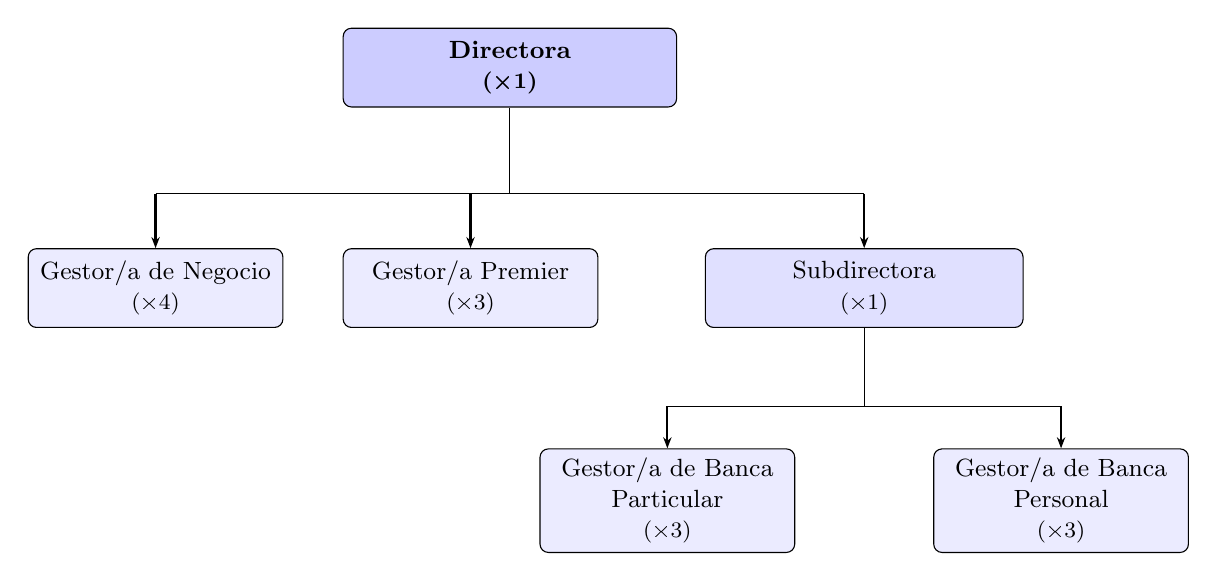
\begin{tikzpicture}[
    box/.style = {
      rectangle, draw, rounded corners = 3pt,
      text width = 3.0cm, align = center,
      minimum height = 1.0cm, font = \small,
      fill = blue!8
    },
    topbox/.style = {
      rectangle, draw, rounded corners = 3pt,
      text width = 4.0cm, align = center,
      minimum height = 1.0cm, font = \small\bfseries,
      fill = blue!20
    },
    midbox/.style = {
      rectangle, draw, rounded corners = 3pt,
      text width = 3.8cm, align = center,
      minimum height = 1.0cm, font = \small,
      fill = blue!12
    },
    arr/.style = {-{Stealth[length=4pt]}, thick}
  ]

  % ---- Nivel 1: Directora ----
  \node[topbox] (dir) at (0,0) {Directora\\{\footnotesize (×1)}};

  % ---- Nivel 2: tres dependencias directas de la Directora ----
  \node[box]    (neg)  at (-4.5,-2.8) {Gestor/a de Negocio\\{\footnotesize (×4)}};
  \node[box]    (prem) at (-0.5,-2.8) {Gestor/a Premier\\{\footnotesize (×3)}};
  \node[midbox] (sub)  at ( 4.5,-2.8) {Subdirectora\\{\footnotesize (×1)}};

  % Barra horizontal nivel 2
  \draw (dir.south) -- (0,-1.6);
  \draw (-4.5,-1.6) -- (4.5,-1.6);
  \draw[arr] (-4.5,-1.6) -- (neg.north);
  \draw[arr] (-0.5,-1.6) -- (prem.north);
  \draw[arr] ( 4.5,-1.6) -- (sub.north);

  % ---- Nivel 3: dependencias de la Subdirectora ----
  \node[box] (bpart) at (2.0,-5.5) {Gestor/a de Banca\\Particular\\{\footnotesize (×3)}};
  \node[box] (bpers) at (7.0,-5.5) {Gestor/a de Banca\\Personal\\{\footnotesize (×3)}};

  % Barra horizontal nivel 3
  \draw (sub.south) -- (4.5,-4.3);
  \draw (2.0,-4.3) -- (7.0,-4.3);
  \draw[arr] (2.0,-4.3) -- (bpart.north);
  \draw[arr] (7.0,-4.3) -- (bpers.north);

  \end{tikzpicture}
  \caption{Organigrama interno de la sucursal de Motril de CaixaBank.
    Fuente: elaboración propia a partir de la entrevista con la directora.}
  \label{fig:organigrama-suc}
\end{figure}

% ===================================================================
\section{Descripción de las unidades y departamentos}
% ===================================================================

A continuación se describe la función de cada unidad o puesto identificado en los
organigramas y se indica a qué parte de la organización pertenece. Las unidades se
agrupan según su papel dentro de la sucursal.

% -------------------------------------------------------------------
\subsection{Ápice estratégico: Directora y Subdirectora de sucursal}
% -------------------------------------------------------------------

El ápice estratégico de la sucursal está formado por la \textbf{Directora} y la
\textbf{Subdirectora}, que concentran la autoridad formal y la responsabilidad última
sobre el funcionamiento de la oficina. No existe línea media interna: entre el ápice
y el núcleo de operaciones no hay ningún nivel jerárquico intermedio, lo que confiere
a la sucursal los rasgos propios de una estructura simple dentro del marco burocrático
que impone CaixaBank desde el exterior.

La \textbf{Directora} es la máxima responsable de la toma de decisiones en la oficina.
Sus funciones abarcan la gestión de los objetivos comerciales locales, la representación
de CaixaBank en el ámbito local y la supervisión directa de los Gestores de Negocio y
los Gestores Premier. Recibe las directrices del Director de Área ---entidad externa a
la sucursal--- y responde ante él de los resultados de la oficina [\ref{ref:entrevista}].

La \textbf{Subdirectora} asiste a la directora y supervisa directamente a los Gestores
de Banca Particular y a los Gestores de Banca Personal, asumiendo las responsabilidades
de dirección en ausencia de la directora.

% -------------------------------------------------------------------
\subsection{Núcleo de operaciones: los equipos de gestores}
% -------------------------------------------------------------------

El personal que atiende directamente a los clientes y ejecuta los servicios financieros
de la sucursal constituye el núcleo de operaciones. La plantilla de 15 personas se
distribuye en cuatro perfiles operativos diferenciados por el segmento de clientela que
atienden [\ref{ref:entrevista}]:

\begin{itemize}

  \item \textbf{Gestor/a de Negocio (×4).}
  Se ocupa de la atención y financiación a pequeñas empresas y autónomos. Sus funciones
  incluyen la instrucción de operaciones de financiación empresarial (préstamos, líneas de
  crédito, descuento comercial), la gestión de cuentas de empresa, el asesoramiento en
  productos de tesorería y el seguimiento de la actividad mercantil del segmento pyme y
  autónomo. Depende directamente de la Directora.

  \item \textbf{Gestor/a Premier (×3).}
  Atiende a clientes con un nivel de ahorro medio-alto que requieren asesoramiento
  financiero especializado. Gestiona productos de ahorro e inversión, seguros, financiación
  hipotecaria y otros productos adaptados al perfil financiero del cliente. Requiere
  habilitación conforme a la normativa MiFID\,II y depende directamente de la Directora.

  \item \textbf{Gestor/a de Banca Particular (×3).}
  Es el puesto de primer contacto con los clientes particulares de la sucursal. Realiza
  las operaciones más habituales del día a día: apertura y mantenimiento de cuentas
  corrientes, gestión de tarjetas, tramitación de transferencias, operativa de caja,
  contratación de productos de ahorro básico y atención de incidencias generales. Depende
  de la Subdirectora.

  \item \textbf{Gestor/a de Banca Personal (×3).}
  Proporciona asesoramiento financiero integral a clientes de alto patrimonio. Sus tareas
  incluyen la planificación patrimonial, la gestión de carteras de inversión, la
  contratación de productos complejos (fondos de inversión, seguros de ahorro, planes de
  pensiones) y el seguimiento personalizado de la situación financiera de cada cliente.
  Requiere habilitación profesional conforme a la normativa MiFID\,II y depende de la
  Subdirectora.

\end{itemize}

% -------------------------------------------------------------------
\subsection{Tecnoestructura: departamentos corporativos de normalización}
% -------------------------------------------------------------------

Desde la perspectiva de la sucursal entendida como unidad autónoma, la tecnoestructura
no forma parte de su estructura interna, sino que constituye un elemento del
\textbf{entorno organizativo} al que se enfrenta la oficina. CaixaBank central actúa
aquí como entorno: impone, desde fuera de la sucursal, las reglas, los procedimientos
y los criterios de actuación que el personal de la oficina debe aplicar en su trabajo
cotidiano. La tecnoestructura es, en consecuencia, la expresión más directa de ese
control externo: un conjunto de departamentos centralizados cuya función no es prestar
servicios directamente a los clientes, sino diseñar, normalizar y controlar los procesos
que rigen la actividad de toda la red de sucursales.

Según confirmó la directora de la sucursal de Motril, ninguno de estos departamentos
cuenta con representación física en la oficina: operan íntegramente desde la sede y su
influencia se materializa a través de los sistemas informáticos, los protocolos internos
y los programas de formación que recibe el personal [\ref{ref:entrevista}]. Esta
ausencia física refuerza la idea de que la tecnoestructura pertenece al entorno y no a
la estructura interna de la sucursal: su control sobre la oficina es real pero mediado,
ejercido a través de normas y sistemas, no de presencia jerárquica directa.
~\\~\\
Su acción sobre la sucursal se concreta en tres formas de normalización. La
\textbf{normalización de procesos} predetermina la secuencia de pasos que el empleado
debe seguir en cada operación ---instrucción de créditos, apertura de cuentas,
comercialización de productos conforme a MiFID\,II--- de modo que la actuación queda
programada con independencia del gestor concreto [\ref{ref:mifid}]. La
\textbf{normalización de habilidades} exige certificaciones profesionales previas ---en
particular la habilitación MiFID\,II para quienes asesoran en inversiones--- antes de
que el empleado pueda ejercer determinadas funciones. La \textbf{normalización de
resultados} fija los parámetros que deben cumplir las operaciones ---modelos de
\textit{scoring}, límites de exposición, garantías exigibles--- acotando la
discrecionalidad del gestor [\ref{ref:basilea}].

% -------------------------------------------------------------------
\subsection{Staff de apoyo: unidades de soporte corporativo}
% -------------------------------------------------------------------

Al igual que la tecnoestructura, el \textit{staff} de apoyo de CaixaBank no forma parte
de la estructura interna de la sucursal, sino que constituye otro componente del
\textbf{entorno organizativo} que CaixaBank central proporciona a la red de oficinas.
Si la tecnoestructura impone restricciones y normaliza comportamientos, el
\textit{staff} de apoyo facilita los recursos y servicios sin los cuales la sucursal no
podría operar: desde la infraestructura tecnológica que sustenta cada transacción hasta
el marco jurídico que encuadra cada contrato. La sucursal utiliza estos servicios, pero
no los diseña ni los controla; le son dados por el entorno del que forma parte.

La directora confirmó que ninguna de estas funciones dispone de representación física en
la sucursal de Motril: operan de forma completamente centralizada desde la sede y prestan
sus servicios a toda la red de oficinas sin intervenir directamente en la atención al
cliente [\ref{ref:entrevista}].
~\\~\\
Entre sus funciones más relevantes para la actividad de la sucursal se encuentran la
gestión de recursos humanos (selección, retribución y movilidad del personal), el
desarrollo y mantenimiento de la infraestructura tecnológica ---\textit{core banking},
CRM y aplicaciones de riesgo--- sobre la que se ejecuta toda la operativa diaria, y el
asesoramiento jurídico en materias contractuales y regulatorias. La sucursal consume
estos servicios como parte de su entorno; no los diseña ni los controla.

\endinput
% -------------------------------------------------------------------
% FIN DEL CAPÍTULO — Julián Carrión Tóbar
% -------------------------------------------------------------------
